\section{Введение}

\subsection{Цель работы}


    Измерить периоды крутильных колебаний рамки при различных положениях закрепленного в ней тела, проверить теорети- ческую зависимость между периодами крутильных колебаний тела относительно различных осей, определить моменты инерции относи- тельно нескольких осей для каждого тела, по ним найти главные моменты инерции тел и построить эллипсоид инерции.


\subsection{В работе используются:}

\begin{itemize}
    \item установка для получения крутильных
колебаний (жесткая рамка, имеющая винты для закрепления в ней твердых тел, подвешенная на натянутой вертикально проволоке);
    \item набор исследуемых твердых тел;
    \item секундомер;
    \item весы;
    \item штангенциркуль.
\end{itemize}

\subsection{Оборудование и их систематические погрешности}

\textbf{Штангенциркуль:} $ \Delta_\text{шт} = 0,1 \text{мм}$

\textbf{Электронные весы:} $ \Delta_\text{в} = 1 \text{г}$

\textbf{Секундомер:} $ \Delta_\text{с} = 0,4 \text{с}$


\section{Теоретические сведения}

\subsection{Экспериментальная установка}
	
	В данной работе используется устройство для получения крутильных колебаний, изображенное на риc. \ref{ris1}. Рамка 1 жестко соединена с проволокой 2, закрепленной вертикально в специальных зажимах 3, позволяющих сообщить начальное закручивание для возбуждения крутильных колебаний вокруг вертикальной оси. В рамке с помощью планки 4, гаек 5 и винта 6 закрепляется твердое тело 7. На теле име- ются специальные выемки, позволяющие его закрепить так, чтобы ось вращения проходила в теле под различными углами через центр масс.

\begin{wrapfigure}{L}{0.3\textwidth}
\centering
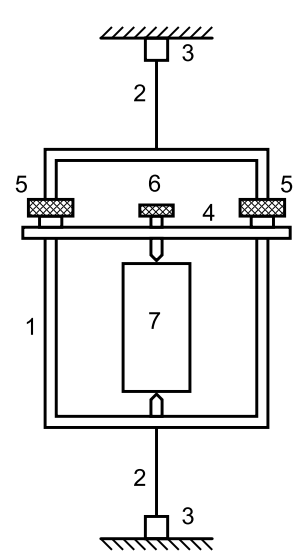
\includegraphics[width=0.3\textwidth]{pictures/ris1.png}
\caption{\label{ris1}Схема установки}
\end{wrapfigure}

Крутильные колебания рамки с телом описываются уравнением
\begin{equation}\label{f1}
		(I + I_p)\frac{d^2\varphi}{dt^2} = -f\varphi.
	\end{equation}
 
 Здесь $І$ и $I_p$ -- моменты инерции тела и рамки относительно оси вращения, $\varphi$ -- угол поворота рамки, меняющийся со временем $t, f$ -- модуль кручения проволоки. Период крутильных колебаний рамки с телом определяется формулой
\begin{equation}\label{f2}
		T = 2\pi \sqrt{\frac{I + I_p}{f}}.
	\end{equation}
 
На рис. \ref{ris2} показано, как проходят оси вращения в параллелепипеде. Оси $AA '$, $BB '$ и $CC '$ являются главными. Моменты инерции относительно этих осей обозначим соответственно $І_x, І_y и I_z$. Ось $DD'$, проходящая вдоль диагонали параллелепипеда, с главными осями составляет такие же углы, как с ребрами $a, b$ и $C$, которые им параллельны. Косинусы этих углов соответственно $A/d, b/d$ и $c/d$, где длина диагонали $d = \sqrt{a^2+b^2+c^2}$.

 \begin{figure}[h]
    \centering
    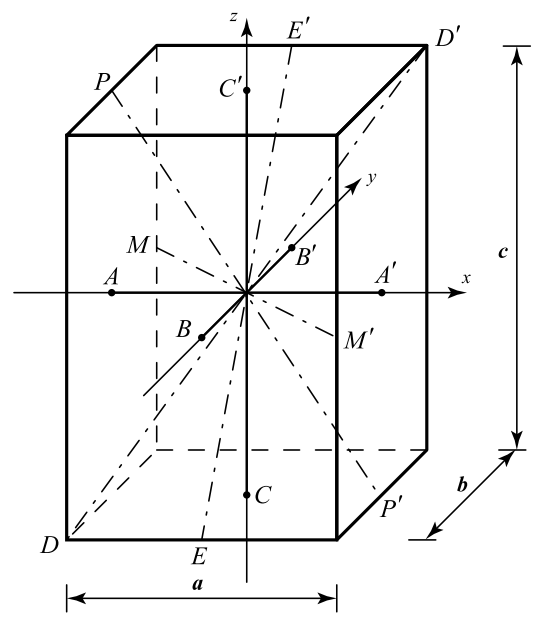
\includegraphics[width=0.45\textwidth]{pictures/ris2.png}
    \caption{Оси вращения прямоугольного параллелепипеда}\label{ris2}
\end{figure} 

Момент инерции $I_d$ при вращении относительно диагонали $DD'$ выражается через главные моменты с помощью следующей формулы:
\begin{equation}\label{f3}
		I_d = I_x \frac{a^2}{d^2} + I_y \frac{b^2}{d^2} + I_z \frac{c^2}{d^2}.
	\end{equation}
 
Отсюда получаем соотношение 
\begin{equation}\label{f4}
		(a^2 + b^2 + c^2)I_d = a^2 I_x  + b^2 I_y + c^2 I_z.
	\end{equation}
 
Используя связь момента инерции с периодом крутильных колебаний \ref{f2}, получаем соотношение между периодами колебаний
\begin{equation}\label{f4}
		(a^2 + b^2 + c^2)T_d^2 = a^2 T_x^2  + b^2 T_y^2 + c^2 T_z^2.
	\end{equation}
 
Экспериментальная проверка этого соотношения является вместе с тем и проверкой соотношения \ref{f3}. Из этой формулы следуют также выражения, связывающие моменты инерции относительно осей $EE$, $MM'$ и $PP$ с главными моментами инерции. С помощью \ref{f2} и для этих осей получаем выражения для периодов крутильных колебаний. Также можно получить следующие формулы
\begin{equation}\label{f4}
		(b^2 + c^2)T_E^2 = b^2 T_y^2 + c^2 T_z^2,
	\end{equation}
 \begin{equation}\label{f4}
		(a^2 + c^2)T_P^2 = a^2 T_x^2 + c^2 T_z^2,
	\end{equation}
 \begin{equation}\label{f4}
		(a^2 + b^2)T_M^2 = a^2 T_x^2  + b^2 T_y^2.
	\end{equation}
 
 Эти соотношения также необходимо проверить экспериментально.

 

 

\newpage